\documentclass[a4paper]{report}

\usepackage[nottoc,numbib]{tocbibind}
\usepackage{graphicx}

\begin{document}

\title{Automatic Structural Inference of Network Protocols}
\author{Fredrik Appelros \and Carl Ekerot}
\date{\today}
\maketitle

\begin{abstract}
An abstract is a brief summary of a research article, thesis, review,
conference proceeding or any in-depth analysis of a particular subject or
discipline, and is often used to help the reader quickly ascertain the paper's
purpose.
\end{abstract}

\tableofcontents

\chapter{Introduction}

\section{Background}
Here we will write a formal introduction to network protocols and why network
protocol inference is needed. Also explain what protocol inference is, of
course.

\section{Related work}
Here is a discussion about related work. We talk about different methodologies
along with their respective advantages and disadvantages. As an example here
is a citation \cite{cui07}.

\chapter{Theory}

\section{Features}
The term feature is explained here and one can draw parallels to how we use
raw data in the K-means example above where that is the most basic kind of
feature.

\subsection{High dimensional data}
Continue to build upon the simple idea of two dimensional clustering and
introduce new problems where the number of dimensions are significantly
higher.

\subsection{Principal component analysis}
Introduce principal component analysis (PCA) and explain how it can relieve
some of the issues that occurs in high dimensional clustering. End with an
example of how this can be done in practice with our choice of features on a
set of data taken from DNS traffic.

\section{Simple linear regression}
In statistics, a response variable $Y_i$ that is linearly dependent on an
explanatory variable $X_i$ can be modeled with a simple linear regression
model. The relationship between the two variables are then

\begin{equation}
    Y_i = \alpha + \beta X_i + \epsilon_i
    \label{eq:slr}
\end{equation}

where $\alpha$ and $\beta$ are the \emph{regression coefficients} and
$\epsilon_i$ is the error term. Given a set of data ${Y_i, X_i}_1^n$ the
regression coefficients can be estimated through simple linear regression. This
process is often called fitting as it can be seen as trying to find the model
with the best fit for the data. There are different methods to do this as there
is no consistent measure for what is the best fit. One common method is the
least squares method.

\subsection{Ordinary least squares}
Ordinary least squares (OLS) is a method for estimating the regression
coefficients in equation~\ref{eq:slr}. It does this by minimizing the sum of
squared residuals of the simple linear regression model. This can be formulated
as minimizing the following cost function.

\begin{equation}
    C(\alpha, \beta) = \sum_{i=1}^n(Y_i - \alpha - \beta X_i)^2
\end{equation}

The result of this is a model that minimizes the residuals \emph{globally}
across all samples. This intrinsically makes the method \emph{non-robust}, i.e.
sensitive to outliers.

\subsection{RANSAC}
Random Sample Consensus (RANSAC) is a \emph{robust} method for fitting a
dataset to a model and was originally intended for image analysis
\cite{fischler81}. The robustness of the method allows it to avoid the
influence of outliers on the model. The algorithm is however
\emph{non-deterministic} meaning that it only produces a good fit with a
certain probability. The solution to this is that the algorithm is normally
run a number of iterations until the probability of success is sufficiently
large.

The model that RANSAC operates on can be any kind of mathematical model, 
therefore when handling two-dimensional linear data the simple linear
regression model given in equation~\ref{eq:slr} can be used. This gives us a
method that solves the problem of simple linear regression but that is also
insensitive to outliers. A comparison between OLS and RANSAC on a dataset where
some samples have been replaced by random noise can be seen in
figure~\ref{fig:ransac}.

\begin{figure}
    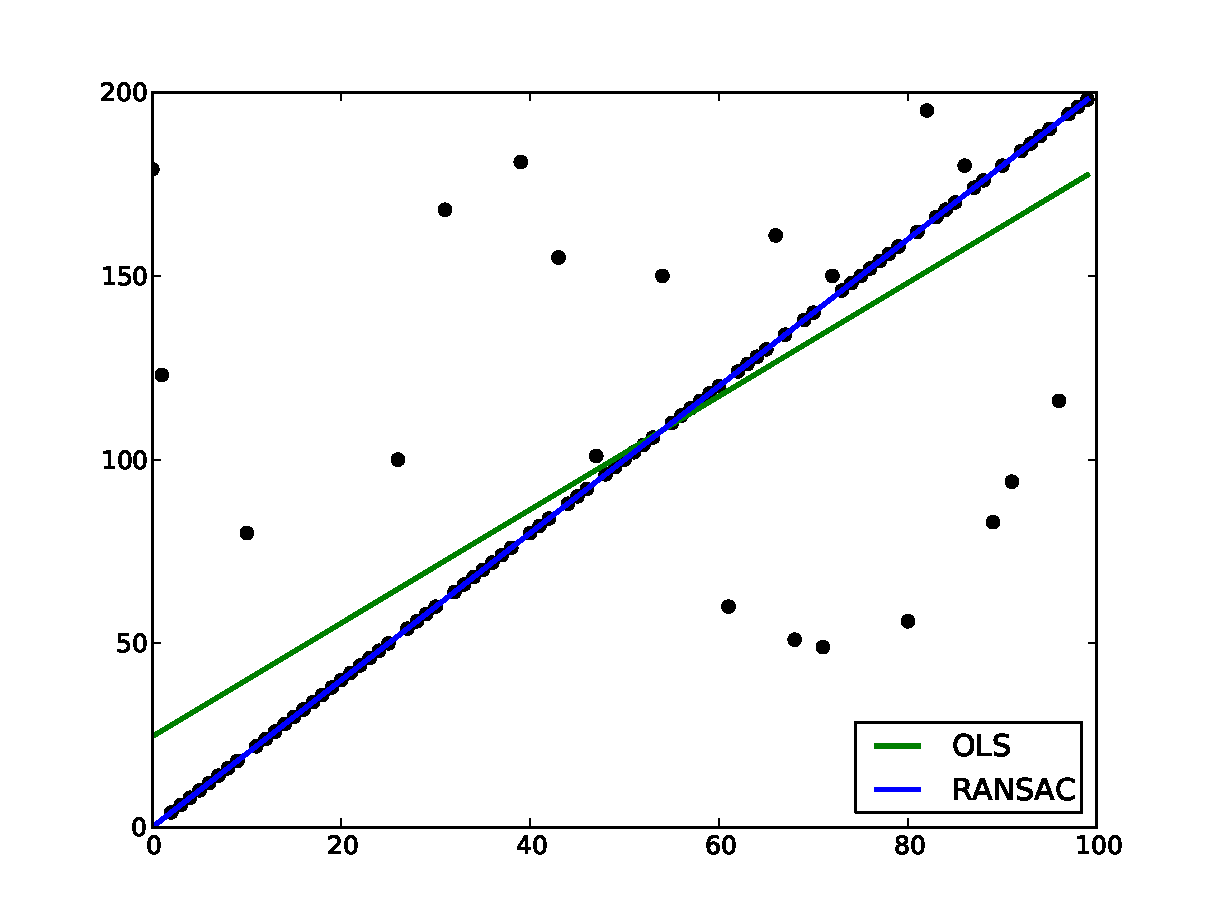
\includegraphics[width=\linewidth]{ransac}
    \caption{The RANSAC algorithm in action.}
    \label{fig:ransac}
\end{figure}

\section{Clustering}
A clustering is a grouping of samples in to individuals \textit{clusters}
based on the similarity of samples based on their features. The features are
predefined to represent distinct properties of the samples. Similarities
between samples are normally represented as distances in an $n$-dimensional
space, where $n$ is the number of features. Distances may be calculated using
a suitable distance function such as euclidean distance. 

In cluster analysis, the goal is normally to find a clustering from a
set of samples such that the membership of a cluster represents some true
relationship. In some clustering algorithms such as K-means, the number of
clusters are predefined \cite{macqueen67}.
When the number of clusters are unknown, other algorithms such as DBSCAN,
OPTICS and hierarchical clustering methods may be used.

The clustering algorithm we use in our method is OPTICS, which is based on
DBSCAN. In the rest of this section we will explain these algorithms and
provide examples based on protocol data.

\subsection{DBSCAN}
Explain the basic idea of density-based clustering. Continue to describe the
DBSCAN algorithm as a practical implementation of the ideas introduced in the
section above. Conclude with an example based on the same DNS data as before.
Be sure to mention the problem with using the method on unknown data as the
parameters needs to be fine tuned.

\subsection{OPTICS}
Introduce the OPTICS algorithm which is an extension to the DBSCAN algorithm
that marries the concepts of hierarchical clustering with density-based
clustering. Emphasize the advantage of more robust parameters but also the
disadvantage of yet again introducing the problem of cluster extraction.

\subsubsection{Cluster extraction}
Explain that the problem with cluster extraction can be solved in OPTICS in
contrast to UPGMA. Start with the most basic threshold extraction and continue
with the more advanced hierarchical extraction method. Conclude with an example
of cluster extraction from DNS data.

\section{Sequence alignment}
Explain the concept of sequence alignment and why it is needed. (We need it
because of fields with variable length)

\subsection{Needleman-Wunsch}
Describe the Needleman-Wunsch algorithm for performing global sequence
alignment.

\section{State machines}
Explain what a state machine is and how it can be represented by an adjacency
matrix.

\chapter{Method}

\section{Approach}
Here we will write how we approached the problem of network protocol inference
and the different components that comprise our method. Start with explaining
why we need to cluster our data and continue to explain what needs to be done
after the clustering step to actually achieve protocol inference.

\section{Type inference}
Explain that our type inference step is actually two different clustering steps
performed in sequence.

\subsection{Initial clustering}
Explain our choice of features and clustering algorithm.

\subsection{Type distinguishers}
Describe our FD clustering algorithm.

\section{Field analysis}
Introduce the classes of fields that we have established as identifiable. Use
plots of their byte distributions to motivate our decision.

\subsection{Byte distribution}
Explain how we reached the decision to use byte distributions in our attempts
to find structures in protocols.

\subsection{Constant fields}

\subsection{Flag fields}

\subsection{Uniform fields}

\subsection{Number fields}

\subsection{Incremental fields}

\subsection{Length fields}
Explain how we use a linear model to model the relationship between length
fields and message lengths.

\section{Protocol state inference}
Explain how we build a state machine from our clusters.

\chapter{Results}

\section{Data sets}
Provide information about the data used to produce the results.

\section{Metrics}
Explain what metrics we use to measure our results.

\section{Clustering performance}
Display the results of applying our method to different data sets.

\section{Field inference performance}

\chapter{Discussion}

\section{Conclusions}
Draw conclusions about our method and compare it to the related methods.

\section{Limitations}
Give a short introduction to the different limitations of our method.

\subsection{Textual protocols}
Explain why our method is not applicable to textual protocols.

\subsection{Variable number of fields}
Explain the problem with protocols that contain a variable number of fields and
why our method does not accomodate for them. (Because we based our definition
of protocols on a fixed number of fields?)

\subsection{Non-aligned data}
Explain why we only try to find aligned fields and the problem with complexity
if we were to relax this requirement.

\subsection{Bit precision}
Talk a little bit about how some protocols do not use entire bytes as the sizes
of their fields and that we will not find exact boundaries for them.

\section{Future work}
Mention the ideas that has come up during the thesis work that we have not had
time to investigate further.

\subsection{Correspondence analysis}
Explain how correspondence analysis could give a better result than PCA.

\subsection{Timestamp identification}
Explain how timestamps could potentially be identified from their distinguished
byte distribution pattern.

\bibliographystyle{plain}
\bibliography{thesis}

\end{document}

